\documentclass[hyperref, a4paper]{article}

\usepackage{geometry}
\usepackage{float}
\usepackage{titling}
\usepackage{titlesec}
% No longer needed, since we will use enumitem package
% \usepackage{paralist}
\usepackage{enumitem}
\usepackage{footnote}
\usepackage{enumerate}
\usepackage{amsmath, amssymb, amsthm}
\usepackage{mathtools}
\usepackage{bbm}
\usepackage{cite}
\usepackage{graphicx}
\usepackage{subcaption}
\usepackage{physics}
\usepackage{tensor}
\usepackage{siunitx}
\usepackage{booktabs}
\usepackage[version=4]{mhchem}
\usepackage{tikz}
\usepackage{xcolor}
\usepackage{listings}
\usepackage{autobreak}
\usepackage[ruled, vlined, linesnumbered]{algorithm2e}
\usepackage{xr-hyper}
\usepackage[colorlinks,unicode]{hyperref} % , linkcolor=black, anchorcolor=black, citecolor=black, urlcolor=black, filecolor=black
\usepackage{prettyref}

% Page style
\geometry{left=3.18cm,right=3.18cm,top=2.54cm,bottom=2.54cm}
\titlespacing{\paragraph}{0pt}{1pt}{10pt}[20pt]
\setlength{\droptitle}{-5em}
\preauthor{\vspace{-10pt}\begin{center}}
\postauthor{\par\end{center}}

% More compact lists 
\setlist[itemize]{itemindent=17pt, leftmargin=1pt}

% Math operators
\DeclareMathOperator{\timeorder}{\mathcal{T}}
\DeclareMathOperator{\diag}{diag}
\DeclareMathOperator{\legpoly}{P}
\DeclareMathOperator{\primevalue}{P}
\DeclareMathOperator{\sgn}{sgn}
\newcommand*{\ii}{\mathrm{i}}
\newcommand*{\ee}{\mathrm{e}}
\newcommand*{\const}{\mathrm{const}}
\newcommand*{\suchthat}{\quad \text{s.t.} \quad}
\newcommand*{\argmin}{\arg\min}
\newcommand*{\argmax}{\arg\max}
\newcommand*{\normalorder}[1]{: #1 :}
\newcommand*{\pair}[1]{\langle #1 \rangle}
\newcommand*{\fd}[1]{\mathcal{D} #1}
\DeclareMathOperator{\bigO}{\mathcal{O}}
\DeclareMathOperator{\object}{Ob}
\DeclareMathOperator{\morphism}{Hom}

% TikZ setting
\usetikzlibrary{arrows,shapes,positioning}
\usetikzlibrary{arrows.meta}
\usetikzlibrary{decorations.markings}
\tikzstyle arrowstyle=[scale=1]
\tikzstyle directed=[postaction={decorate,decoration={markings,
    mark=at position .5 with {\arrow[arrowstyle]{stealth}}}}]
\tikzstyle ray=[directed, thick]
\tikzstyle dot=[anchor=base,fill,circle,inner sep=1pt]

% Algorithm setting
% Julia-style code
\SetKwIF{If}{ElseIf}{Else}{if}{}{elseif}{else}{end}
\SetKwFor{For}{for}{}{end}
\SetKwFor{While}{while}{}{end}
\SetKwProg{Function}{function}{}{end}
\SetArgSty{textnormal}

\newcommand*{\concept}[1]{{\textbf{#1}}}

\newrefformat{fig}{Figure~\ref{#1}}

% Embedded codes
\lstset{basicstyle=\ttfamily,
  showstringspaces=false,
  commentstyle=\color{gray},
  keywordstyle=\color{blue}
}

\title{Quantum Optics, Homework 3}
\author{Jinyuan Wu}

\begin{document}

\maketitle

\begin{figure}
    \centering
    \tikzset{every picture/.style={line width=0.75pt}} %set default line width to 0.75pt        

\begin{tikzpicture}[x=0.75pt,y=0.75pt,yscale=-1,xscale=1]
%uncomment if require: \path (0,319); %set diagram left start at 0, and has height of 319

%Image [id:dp6954457554746387] 
\draw (280.94,160.96) node  {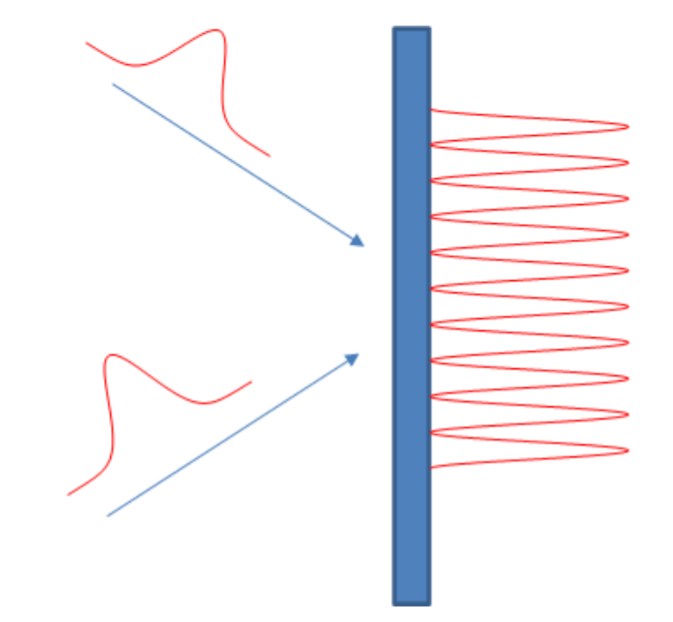
\includegraphics[width=162.44pt,height=162.44pt]{problem-1-detector.PNG}};
%Straight Lines [id:da9771961350544831] 
\draw    (138,41.86) -- (443.02,41.86) ;
\draw [shift={(445.02,41.86)}, rotate = 180] [fill={rgb, 255:red, 0; green, 0; blue, 0 }  ][line width=0.08]  [draw opacity=0] (12,-3) -- (0,0) -- (12,3) -- cycle    ;
%Straight Lines [id:da46670676444957326] 
\draw    (138,281) -- (138,41.86) ;
\draw [shift={(138,283)}, rotate = 270] [fill={rgb, 255:red, 0; green, 0; blue, 0 }  ][line width=0.08]  [draw opacity=0] (12,-3) -- (0,0) -- (12,3) -- cycle    ;

% Text Node
\draw (447.02,41.86) node [anchor=west] [inner sep=0.75pt]    {$z$};
% Text Node
\draw (138,286.4) node [anchor=north] [inner sep=0.75pt]    {$x$};


\end{tikzpicture}
    \caption{The two Gaussian beams incident to a detector}
\end{figure}

\paragraph{Interference between Gaussian pulses} Consider two Gaussian pulses with wave vectors
$\boldsymbol{k}_{1,2}=k(\pm \sin \theta, 0, \cos \theta)$, respectively.
They are incident to a plane detector on the surface $z=0$. 
The intensity distributions of the two beams are all 
\begin{equation}
    |\mathcal{E}|^{2} \propto e^{-\left(x^{2}+y^{2}\right) / \sigma^{2}},
\end{equation} 
with $\sigma \gg \lambda$. The pulses arrive at the detector simultaneously.
The detector absorbs the pulses completely and there is no reflection.
Calculate $P^{(1)}(\vb*{r})$ and $P^{(2)}(\vb*{r}_1, \vb*{r}_2)$ for the following states of the optical field: 
\begin{itemize}
    \item[(a)] $|\psi\rangle=\frac{1}{\sqrt{2^{N} N !}}\left(a_{1}^\dagger+a_{2}^\dagger\right)^{N}|V\rangle$.
    \item[(b)] $|\psi\rangle=\frac{1}{N !}\left(a_{1}^\dagger a_{2}^\dagger\right)^{N}|V\rangle$.
    \item[(c)] $|\psi\rangle=\frac{1}{\sqrt{2 N !}}\left(\left(a_{1}^\dagger\right)^{N}+\left(a_{2}^\dagger\right)^{N}\right)|V\rangle$.
    \item[(d)] $|\psi\rangle=D_{1}(\alpha) D_{2}(\alpha)|V\rangle, \quad D_{j}(\alpha) \equiv e^{\alpha a_{j}^\dagger-\alpha^{*} a_{j}}$.
    \item[(e)] $|\psi\rangle=\frac{1}{\sqrt{2}}\left(D_{1}(\alpha)+D_{2}(\alpha)\right)|V\rangle$.
\end{itemize}

\paragraph{Solution} The electric field operator is 
\begin{equation}
    \vb*{E} = \sum_{i=1, 2} \vb*{\mathcal{E}}_i \ee^{\ii \vb*{k}_i \cdot \vb*{r} - \ii \omega t} a_i + \text{h.c.}. 
\end{equation}
\begin{itemize}
\item[(a)] We define 
\[
    b^\dagger = \frac{1}{\sqrt{2}} (a_1^\dagger + a_2^\dagger),
\] 
and now the wave function is 
\[
    \ket*{\psi} = \frac{1}{\sqrt{N!}} (b^\dagger)^N \ket*{0}.
\]
We have 
\[
    P^{(1)}(\vb*{r}) = \frac{1}{N!} \abs*{\vb*{\mathcal{E}} (\vb*{r})}^2 
    \expval*{b^N (a_1^\dagger a_1 + a_2^\dagger a_2 + \ee^{\ii (\vb*{k}_2 - \vb*{k}_1) \cdot \vb*{r}} a_1^\dagger a_2 + \ee^{\ii (\vb*{k}_1 - \vb*{k}_2) \cdot \vb*{r}} a_2^\dagger a_1 ) (b^\dagger)^N}{0} .
\]
Evaluating the terms in the RHS above, we have 
\[
    \begin{aligned}
        \expval*{b^N a_1^\dagger a_1 (b^\dagger)^N}{0} &= N \expval*{b a_1^\dagger}{0} \times N \expval*{a_1 b^\dagger}{0} 
        \times \text{contraction of $(N-1)$ $b$'s and $(N-1)$ $b^\dagger$'s} \\
        &= N \expval*{b a_1^\dagger}{0} \times N \expval*{a_1 b^\dagger}{0} \times (N-1)! \expval*{b b^\dagger}{0} \\
        &= N \times \frac{1}{\sqrt{2}} \times N \frac{1}{\sqrt{2}} \times (N-1)! \times 1 = \frac{1}{2} N^2 (N-1)!,
    \end{aligned}
\]
and similarly 
\[
    \expval*{b^N a_2^\dagger a_2 (b^\dagger)^N}{0} = \frac{1}{2} N^2 (N-1)!,
\]
and 
\[
    \begin{aligned}
        \expval*{b^N a_1^\dagger a_2 (b^\dagger)^N}{0} &= N \expval*{b a_1^\dagger}{0} \times N \expval*{a_2 b^\dagger}{0} 
        \times \text{contraction of $(N-1)$ $b$'s and $(N-1)$ $b^\dagger$'s} \\
        &= N \expval*{b a_1^\dagger}{0} \times N \expval*{a_2 b^\dagger}{0} \times (N-1)! \expval*{b b^\dagger}{0} \\
        &= N \times \frac{1}{\sqrt{2}} \times N \frac{1}{\sqrt{2}} \times (N-1)! \times 1 = \frac{1}{2} N^2 (N-1)!,
    \end{aligned}
\]
and similarly 
\[
    \expval*{b^N a_1^\dagger a_2 (b^\dagger)^N}{0} = \frac{1}{2} N^2 (N-1)!.
\]
Putting everything together we have 
\[
    \begin{aligned}
        P^{(1)}(\vb*{r}) &= \frac{1}{N!} \abs*{\vb*{\mathcal{E}} (\vb*{r})}^2 \times \frac{1}{2} N^2 (N-1)! 
        \times (2 + \ee^{\ii (\vb*{k}_2 - \vb*{k}_1) \cdot \vb*{r}} + \ee^{\ii (\vb*{k}_1 - \vb*{k}_2)) \cdot \vb*{r} }) \\
        &= N \abs*{\vb*{\mathcal{E}}(\vb*{r})}^2 (1 + \cos (\vb*{k}_1 - \vb*{k}_2) \cdot \vb*{r}),
    \end{aligned}
\]
so finally 
\begin{equation}
    P^{(1)}(\vb*{r}) = N \abs*{\vb*{\mathcal{E}}(\vb*{r})}^2 (1 + \cos (\vb*{k}_1 - \vb*{k}_2) \cdot \vb*{r}) \propto N \ee^{- (x^2 + y^2) / \sigma^2} (1 + \cos (\vb*{k}_1 - \vb*{k}_2) \cdot \vb*{r}).
\end{equation}

\item[(b)] We have 
\[
    \begin{aligned}
        P^{(1)}(\vb*{r}) &= \frac{1}{(N!)^2} \expval*{(a_2 a_1)^N (a_1^\dagger a_1 + a_2^\dagger a_2 + \ee^{\ii (\vb*{k}_2 - \vb*{k}_1) \cdot \vb*{r}} a_1^\dagger a_2 + \ee^{\ii (\vb*{k}_1 - \vb*{k}_2) \cdot \vb*{r}} a_2^\dagger a_1 ) (a_1^\dagger a_2^\dagger)^N}{0} \\
        &= 
    \end{aligned}
\] 
  
\item[(c)] 
\end{itemize}

\paragraph{}

\end{document}